\documentclass{article}
\usepackage[utf8]{inputenc}
\usepackage[margin = 1.1in, headheight = 0.9in, footskip = 0.75 in]{geometry}
\usepackage{fancyhdr}
\usepackage{lastpage}
\usepackage{amsmath}
\usepackage{amssymb}
\usepackage{xparse}
\usepackage{graphicx}
\usepackage{enumerate}
\usepackage{mathtools}
\usepackage{amsthm}
\usepackage{tikz-cd}
\usepackage{tikz}
\usepackage{array}
\usepackage{pgfplots}
\usepackage{bbm}
\usepackage[shortlabels]{enumitem}
\usepackage{algorithm}
\usepackage{algpseudocode}
\usepackage{booktabs}
\usepackage{hyperref}
\hypersetup{
    colorlinks=true,
    linkcolor=black,
    filecolor=magenta,      
    urlcolor=red
    }

\urlstyle{same}
\newcommand{\RNum}[1]{\uppercase\expandafter{\romannumeral #1\relax}}
\newcommand\ddfrac[2]{\frac{\displaystyle #1}{\displaystyle #2}}
\usepackage{xpatch}
\setlength{\parindent}{3em}
\setlength{\parskip}{0.5em}
\newcolumntype{C}{>{\centering\arraybackslash}p{1cm}}
%===================================================================================================
\pagestyle{fancyplain}
\renewcommand{\headrulewidth}{0pt}
\renewcommand{\footrulewidth}{0pt}
\fancyhf{}\par 
\lhead{\hspace{0cm}\\\hspace{0cm}\\Zmh6339\\AI \& Machine Learning, CS-UH 3260\\Professor Keith Ross}
\rhead{Ziad Hassan\\ February 12, 2024}
\cfoot{\thepage/\pageref{LastPage}}
%===================================================================================================
\title{Assignment 2}
\date{}
\author{}
%===================================================================================================
\begin{document}
\maketitle
%==================================================================================================
\section*{Question 1}
Below is the plotting of $Q(\texttt{s,stick})$\\ 
where $s\coloneq(\texttt{player total} = 18, \texttt{dealer showing} = 8, \texttt{no usable ace})$
in the first MCES version of the Blackjack game over 10,000 epsiodes (where every 100th episode was recorded).
\begin{center}
    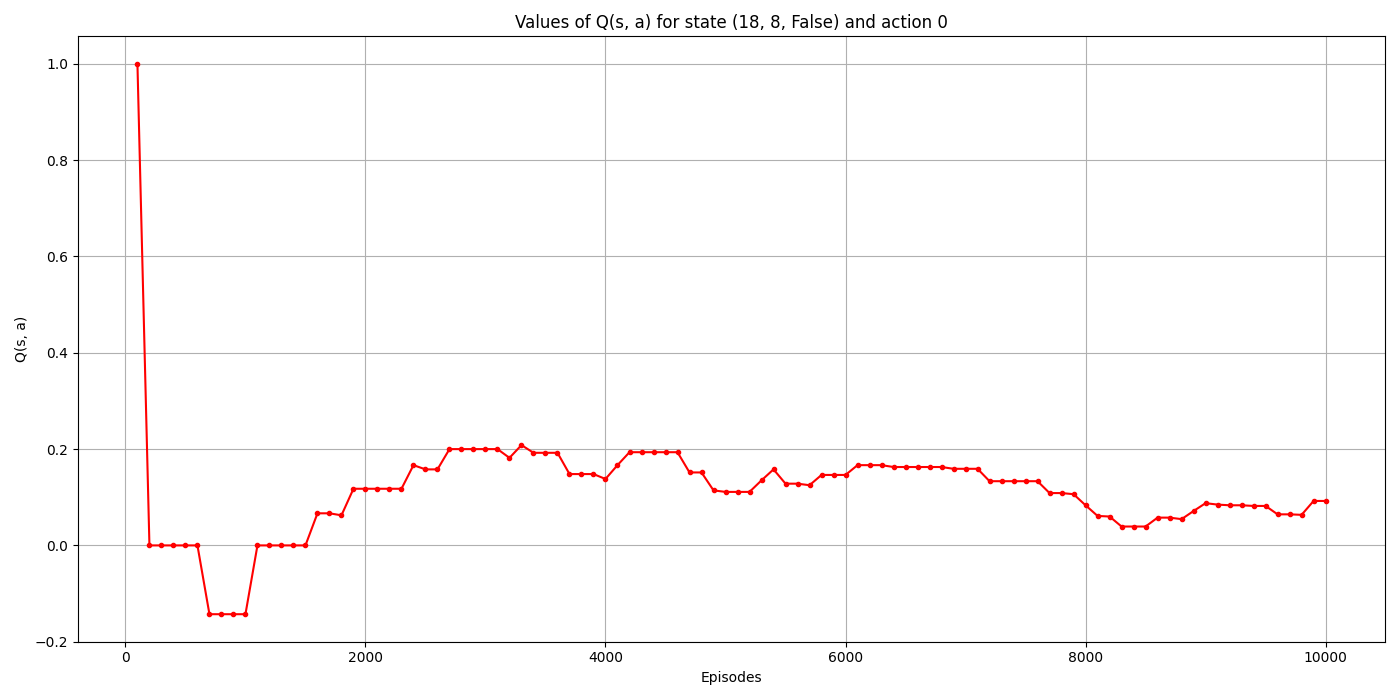
\includegraphics[scale=0.5]{Q_values.png}
\end{center}
%==================================================================================================
\section*{Question 2}
Below is the plotting of $Q(\texttt{s,stick})$\\ 
where $s\coloneq(\texttt{player total} = 18, \texttt{dealer showing} = 8, \texttt{no usable ace})$
in the second MCES version of the Blackjack game over 10,000 epsiodes (where every 100th episode was recorded).
\begin{center}
    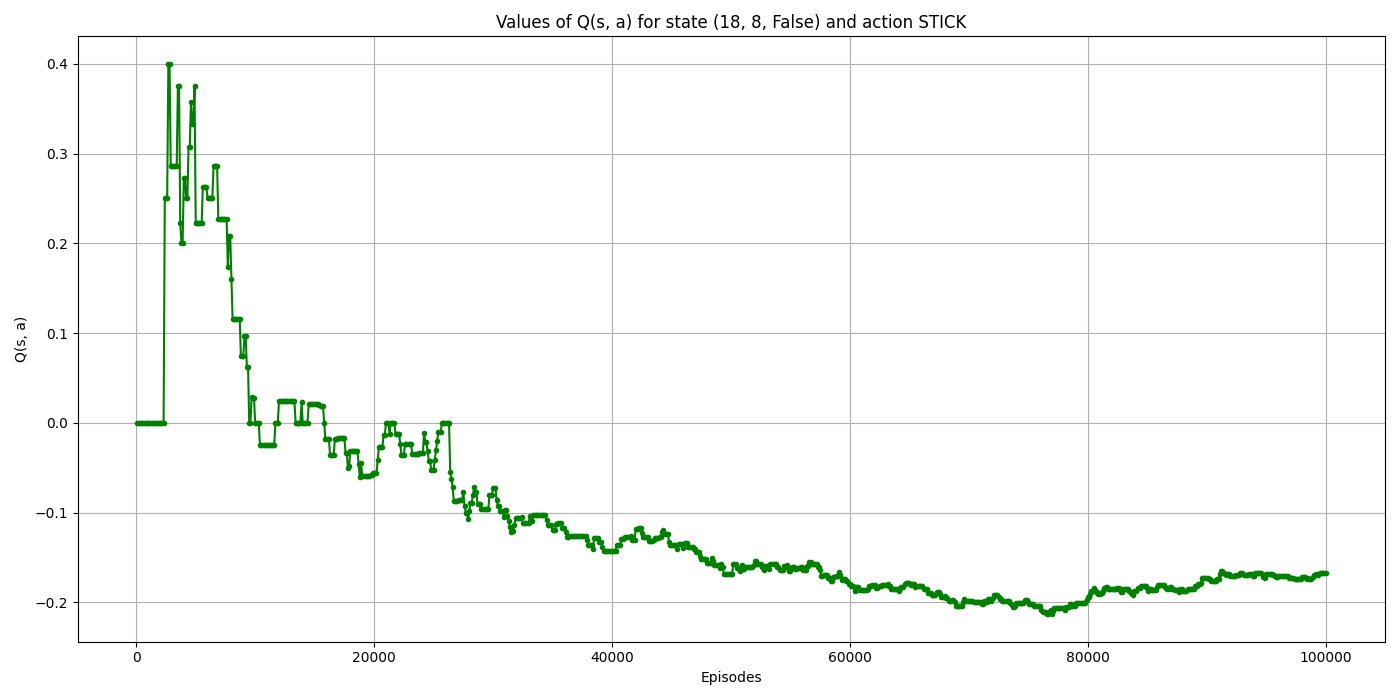
\includegraphics[scale=0.5]{Q_values2.png}
\end{center}
%==================================================================================================
\end{document}